\chapter{State-of-the-Art}

\section{Evolution of TA-definitions}

Several attempts were made to formally define the timing anomaly. Here we give a review of some definitions which can be applied to our architecture model.

\subsection{Step Heights}

Gebhard \cite{gebhard_timing_2012} gives a timing-anomaly definition based on local execution time of instruction in comparison to global execution time defined as sum of local ones. TA exists when local execution time of earlier instruction is lower and the global execution time of some later instruction is higher (compared to other trace).

Figure \ref{fig:step-good} shows this definition applied to example \ref{ex:simple-ta}. Orange arrow illustrates the local execution time of instruction $A$. The global time for instruction $D$ is different between traces $\alpha$ and $\beta$ (13 and 11 respectively).

\begin{figure}[!htb]
    \centering
    \begin{subfigure}[t]{0.5\textwidth}
        \centering
        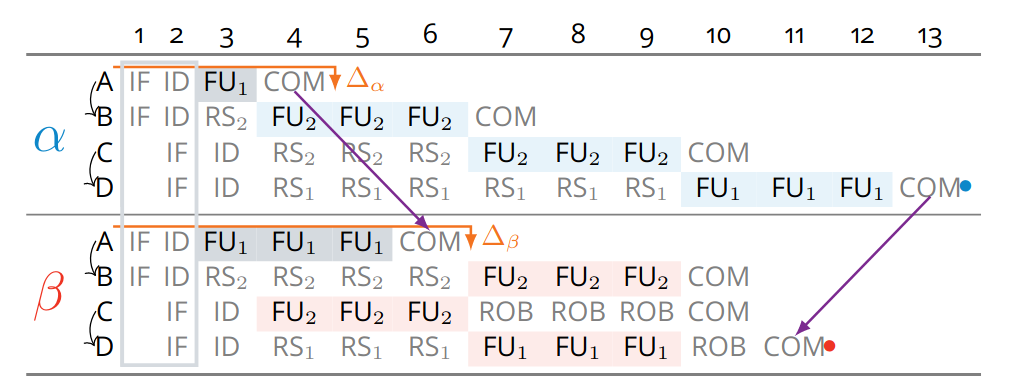
\includegraphics[width=\textwidth]{figures/step-func-good.png}
        \caption{Interpretation of example \ref{ex:simple-ta} using Gebhard's definition}
        \label{fig:step-good}
    \end{subfigure}
    \hfill
    \begin{subfigure}[t]{0.49\textwidth}
        \centering
        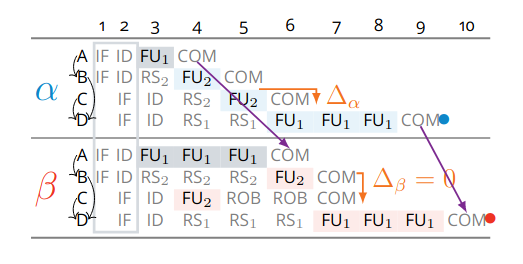
\includegraphics[width=\textwidth]{figures/step-func-bad.png}
        \caption{Counterexample to the definition}
        \label{fig:step-bad}
    \end{subfigure}
    \caption{Gebhard's definition applied to execution traces (from \cite{binder_definitions_2022})}
    \label{fig:step}
\end{figure}

In his thesis \cite{binder_definitions_2022}, Binder provides a counterexample (figure \ref{fig:step-bad}), where it is clear that there is no TA (trace $\beta$ has both unfavorable variation and longer execution time). However, the Gebhard's definition signals an anomaly because of shorter local execution time of instruction $C$ in trace $\beta$.

This poses a question whether it is reasonable to capture a local execution time as difference between instruction complitions. 

\subsection{Step-functions Intersections}

Similar definition is proposed by Cassez et al. \cite{cassez_what_2012}. The difference is that only global execution time is taken into account. Thus, TA arises when step-functions (that map instructions to their absolute completion time) of two traces intersect. 

\begin{figure}[!htb]
    \centering
    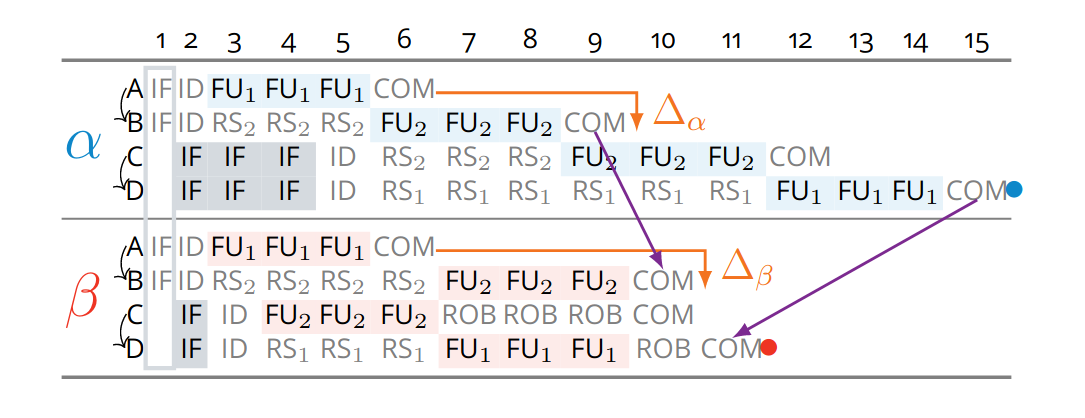
\includegraphics[width=\textwidth]{figures/step-func-2-bad.png}
    \caption{Contradicting result of Cassez's definition (from \cite{binder_definitions_2022})}
    \label{fig:step-2}
\end{figure}

This definition also leads to misleading effect where scenario \cite{binder_definitions_2022} where it is clear that no time anomaly is present, but it is still detected by the definition. Figure \ref{fig:step-2} illustrates this contradiction. \TODO{details}

\subsection{Component Occupation}

An alternative approach is proposed by Kirner et al. \cite{kirner_precise_2009}. In their work the idea is to partition hardware into components and for each define the occupation by instruction (for how many cycles it processes the instruction). TA arises when a shorter component occupation coincides with a longer execution time in a chosen trace. However, as is shown is \cite{binder_definitions_2022} the results depend on how we define component partition which imposes the major concern against using this definition.

\subsection{Instruction Locality}
\subsection{Progress-based definition}

Hahn and Reineke \cite{hahn_design_2020} intorduce the notion of progress, ... \cite{gruin_minotaur_2023}

\subsection{Event Time Dependency Graph}



\section{TA-classifications}

